%%%%%%%%%%%%%%%%%%%%%%%%%%%%%%%%%%%%%%%%%%%%%%%%%%%%%%%%%%%%%%%%%%%%%%%%
%
%
%     This file is included from the file   Segmentation.tex
% 
%     Section tag and label are placed in this top file.
%
%
%
%%%%%%%%%%%%%%%%%%%%%%%%%%%%%%%%%%%%%%%%%%%%%%%%%%%%%%%%%%%%%%%%%%%%%%%%



\piccaption[Zero Set Concept]{Concept of Zero Set in a Level Set.\label{fig:LevelSetZeroSet}}
\parpic(9cm,6cm)[r]{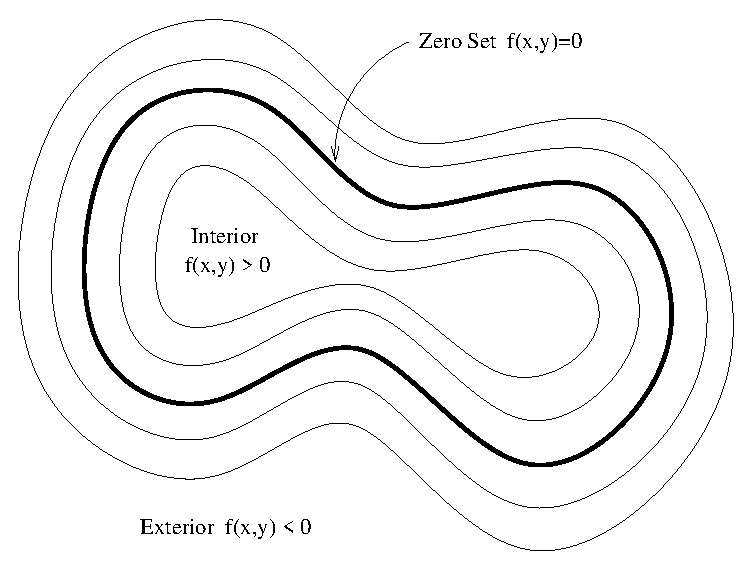
\includegraphics[width=8cm]{LevelSetZeroSet.eps}}

The paradigm of Level Set is a numerical method for tracking the evolution of
contours and surfaces. Instead of manipulating the contour directly, the
contour is embedded as the zero level set of a higher dimensional function
called the level set function, $\psi(\bf{X},t)$. The level set function is then
evolved under the control of a differential equation. At any time, the evolving
contour can be obtained by extracting the zero level set $\Gamma(\bf(X),t) =
\{\psi(\bf{X},t) = 0\}$.  The main advantages of using levels sets is that
arbitrarily complex shapes can be modeled and topologically changes such as
mergeing and splitting is handled implicitly.

Level sets can be used for image segmentation by using image based features such
as mean intensity, gradient and edges in the governering differential equation. 
In a typical approach, a contour is initialized by a user and then is evolved 
until it fits to the form of an anatomical structure in the image. 
Many different implementation and variants of this basic concept have been
published in the literature. A overview of the field has been made by Sethian
\cite{Sethian1996}. The following sections introduce practical examples of some
of the Level Set segmentation methods available in ITK.


\subsection{Fast Marching Segmentation}
\label{sec:FastMarchingImageFilter}

\ifitkFullVersion
\input{FastMarchingImageFilter.tex}
\fi



\subsection{Shape Detection Segmentation}
\label{sec:ShapeDetectionLevelSetFilter}

\ifitkFullVersion
\input{ShapeDetectionLevelSetFilter.tex}
\fi


\subsection{Geodesic Active Contours Segmentation}
\label{sec:GeodesicActiveContourImageFilter}

\ifitkFullVersion
\input{GeodesicActiveContourImageFilter.tex}
\fi



\subsection{Threshold Level Set Segmentation}

\subsection{Segmentation Level Set Image Filter}
\label{sec:SegmentationLevelSetImageFilter}


